%==============================================================================
% SBR/LARS 2026 (Robotica 2026, Joao Pessoa) -- camera-ready of submission
% #34344 (JEMS). Template: IEEEtran (conference), A4.
%
% Camera-ready changes (2026-09-23): see paper/sbr2026_camera_ready/CAMERA_READY_NOTES.md
% in the digitaltwin repository. Every number in the text comes from a
% repository artifact cited in a "% source:" comment next to it.
%
% Before submitting: the checklist greps for REPLACE-ME and must find nothing
% (authors, affiliation, e-mails, acknowledgment, repository URL, video URL).
%
% Build: pdflatex main && bibtex main && pdflatex main && pdflatex main
%==============================================================================
\documentclass[conference,a4paper]{IEEEtran}
\IEEEoverridecommandlockouts
\usepackage{cite}
\usepackage{amsmath,amssymb,amsfonts}
\usepackage{graphicx}
\usepackage{textcomp}
\usepackage{xcolor}
\usepackage{booktabs}
\usepackage{siunitx}
\usepackage{url}
\usepackage{tikz}
\usetikzlibrary{arrows.meta,positioning,fit,backgrounds,calc}
\usepackage{stfloats}   % figure*/table* at the bottom; avoids floats pushed past the references
\graphicspath{{figures/}}

% --- Float placement -----------------------------------------------------
\setcounter{topnumber}{3}
\setcounter{bottomnumber}{2}
\setcounter{totalnumber}{4}
\renewcommand{\topfraction}{0.92}
\renewcommand{\bottomfraction}{0.85}
\renewcommand{\textfraction}{0.07}
\renewcommand{\floatpagefraction}{0.70}

\def\BibTeX{{\rm B\kern-.05em{\sc i\kern-.025em b}\kern-.08em
    T\kern-.1667em\lower.7ex\hbox{E}\kern-.125emX}}

% --- Notation shortcuts -------------------------------------------------------
\newcommand{\epos}{e_{\mathrm{pos}}}
\newcommand{\eang}{e_{\mathrm{ang}}}
\newcommand{\SEtwo}{\mathrm{SE}(2)}
\newcommand{\Td}{T_{d}}

% --- Page budget switch ------------------------------------------------------
% Fig. "trajectory overlays by label" (figure*, ~0.3 page) is left out so that the
% camera-ready fits 6 pages with the new robot/measurement-chain figure. Set to
% \keeptrajfigtrue if the JEMS page limit allows a 7th page.
\newif\ifkeeptrajfig \keeptrajfigfalse

% --- Camera-ready links (fill both; the checklist greps for REPLACE-ME) -------
% Repository: public GitHub release of the reproduction package (+ Zenodo DOI).
% Videos: supplementary videos (YouTube unlisted or Zenodo).
\newcommand{\repolink}{\url{https://REPLACE-ME}}
\newcommand{\videolink}{\url{https://REPLACE-ME}}

\begin{document}

% Title as registered in JEMS (kept by the author on 2026-09-23). If the title is
% changed, JEMS and this line must match.
\title{A Behavioral Model for Reality-Gap Mitigation in Digital Twins of Omnidirectional Soccer Robots}

% Author list and order exactly as registered in JEMS.
\author{\IEEEauthorblockN{REPLACE-ME First Author\IEEEauthorrefmark{1},
REPLACE-ME Co-author\IEEEauthorrefmark{1}}
\IEEEauthorblockA{\IEEEauthorrefmark{1}Centro de Inform\'atica, Universidade Federal de Pernambuco (CIn-UFPE), Recife, Brazil\\
Rob\^{o}CIn Robotics Team\\
Email: \{REPLACE-ME\}@cin.ufpe.br}}

% IEEE copyright line: enable only if the organizers send the exact text.
% \IEEEpubid{\makebox[\columnwidth]{979-8-XXXX-XXXX-X/26/\$31.00~\copyright2026 IEEE\hfill}%
%   \hspace{\columnsep}\makebox[\columnwidth]{ }}

\maketitle

%==============================================================================
% ABSTRACT -- camera-ready (2026-09-23): one paragraph, as reviewer R2 asked.
% IEEE: no math symbols, no citations. Numbers unchanged from the reviewed version:
% 87% (CHANGELOG 2026-06-14); 71.1% (results/identificacao_omega_20260724.md);
% 1% and 56% (results/omega_excitation_analysis_20260807_133917.json,
% results/excitation_per_dof_20260810_1022.md); 0.039/0.101/0.129 and 73.5 s
% (results/epos_eang_three_models_20260810_1022.md, results/clustered_stats_20260809_2309.md);
% ablation (results/ablation_orderfree_20260810_1021.md); 99.6% (Sec. IV-B,
% results/bin_distribution_20260724_155551.md).
%==============================================================================
\begin{abstract}
Teams in the RoboCup Small Size League develop and validate control software largely in simulation, where simplified physics leaves a reality gap to the field. This paper asks which behavioral model of an omnidirectional soccer robot can be identified from the competition logs teams already record, and what those logs cannot supply. Each body-frame degree of freedom is modeled as a first-order-plus-dead-time channel. The two translational channels are identified from in-game logs and reach roughly 87 percent hold-out fit. The yaw channel is not: during play the yaw command carries a median of one percent of the per-wheel actuation and explains only 56 percent of the measured rotation, so a short dedicated open-loop campaign restores the excitation and identifies the channel at 71 percent hold-out fit. Fidelity is evaluated in free run over horizons of 0.1 to 1.5 seconds, with every plant in the same harness. Over 73.5 seconds of held-out motion from ten events, the model reaches a median position error of 0.039 meters at the 0.4-second horizon, against 0.101 for ideal kinematics and 0.129 for rSim, the ODE engine of the rSoccer framework, run untuned and reported as context. The model is lower in all ten events, and an order-independent ablation attributes the gain in comparable parts to the time constant and the dead time, conditional on the measured initial velocity. Because 99.6 percent of the hold-out windows are translation-dominated, rotational fidelity remains unvalidated; a screening computable from the logs alone predicts which channels a log can identify.
\end{abstract}


\begin{IEEEkeywords}
digital twin, system identification, robot modeling, omnidirectional robot, robot soccer
\end{IEEEkeywords}

%==============================================================================
% INTRODUCTION — corte 9->6 paginas (2026-08-10, pedido do autor).
%  - 4o paragrafo ("This paper models...") REMOVIDO: repetia o abstract e as
%    contribuicoes. O essencial (o que e medido, contra o que) migrou para uma
%    frase de fecho do 3o paragrafo.
%  - Contribuicoes: maximo 2 frases cada.
% Todas as citacoes preservadas. Nenhuma referencia removida.
%==============================================================================
\section{Introduction}
\label{sec:intro}

The RoboCup Small Size League (SSL) fields teams of fast, omnidirectional, four-wheeled robots whose coordination software is written, tuned, and regression-tested almost entirely on simulators. The league's reference simulation tools implement a simplified omnidirectional wheel model on top of a rigid-body ODE engine \cite{monajjemi2012grsim}; reinforcement-learning frameworks inherit that engine \cite{martins2021rsoccer}; and recent motion-planning policies for the SSL are trained in these environments \cite{machado2025planning}. Because the simulated dynamic response departs from that of the physical robot, behavior that passes validation in simulation often degrades once deployed. This discrepancy is what the literature calls the reality gap.

Recent efforts to narrow it converge on \emph{digital twins}: simulation models bound to one specific physical asset and kept faithful to it by data measured from that asset, rather than generic models of a class of robots. Twins of mobile platforms have been built for commercial AGVs \cite{barioni2024development}, and for the navigation and control of omnidirectional robots \cite{yang2025digital}, and grey-box identification has been evaluated as the module that produces the model within such a twin \cite{brennan2025greybox}. Building one is not free: it normally presumes either a detailed physical description of the mechanism, whose mechanical parameters teams rarely have, or
a dedicated excitation campaign, which demands the robot, the field, and time outside of competition.

Competition logs are an attractive alternative because teams already record them: body-frame velocity commands and vision poses at roughly \SI{60}{Hz} during closed-loop play. Existing work, however, reflects the difficulty of using them by avoiding it. Simulation models of omnidirectional platforms are
tuned on dedicated real trajectories \cite{wiedemann2024simulation,wiedemann2025automated}, identification pipelines design excitation sequences per parameter group \cite{giro2023otbot}, real-time
estimation for twins assumes informative operating data \cite{kosmaga2026digital}, and offline sim-to-real calibration presumes the pre-collected data excite the parameters of interest \cite{tiboni2023dropo}. Whether a behavioral model can be identified from closed-loop \emph{operational} logs, and which degrees of freedom (DOF) such logs support, remains underexplored. This paper answers that question for an SSL robot modeled as three decoupled first-order-plus-dead-time (FOPDT) channels, one per DOF, evaluated in free run against a zero-parameter baseline under an identical harness.

\noindent\textbf{Contributions.}
\textbf{(C1)} A per-DOF grey-box FOPDT identification methodology for an omnidirectional robot from \emph{closed-loop} competition logs, validated on held-out events, for the degrees of freedom those logs excite. 
\textbf{(C2)} A fidelity protocol that scores the model the way it is used: driven only by the recorded commands from a known pose, with no correction from measured data inside the window. Verdicts are issued per motion regime and only when a paired test, an effect size, and a bootstrap interval agree.
% source: src/dtssl/sim/rollout.py ; src/dtssl/eval/metrics.py ; config/metrics.json
\textbf{(C3)} A translational fidelity result with the improvement attributed to its source: the model lowers the median position error of the baseline in all ten hold-out events, and an order-independent ablation splits the effect between the time constant and the dead time, conditional on the measured initial state.
\textbf{(C4)} A pre-fit screening procedure that predicts, from an operational log alone, which degrees of freedom that log can identify. It combines two quantities computable before any model is estimated: the share of the actuation each command carries and the variance of the attained velocity it explains. On this robot it separates the identifiable channels from the unidentifiable one before a single parameter is fitted.
% source: results/omega_excitation_analysis_20260807_133917.json
\section{Related Work}
\label{sec:related}

\subsection{Behavioral twins of mobile robots}
Digital twins of mobile platforms are typically validated behaviorally, by comparing simulated and real trajectories rather than parameters \cite{barioni2024development,yang2025digital}. On the construction side, grey-box identification has been assessed as the model-generating module of a twin and has been found to be sensitive to the informativeness of its input data \cite{brennan2025greybox}. Work on omnidirectional platforms assumes dedicated experiments, whether one experiment per parameter group \cite{giro2023otbot} or tuning against motion-capture trajectories, manually and per trajectory
\cite{wiedemann2024simulation}, or by black-box optimization over a few high-impact parameters \cite{wiedemann2025automated}. The per-DOF FOPDT structure adopted here is the classic first-order-plus-dead-time process model of control practice \cite{astrom1995pid}. The closest precedent for reusing
data that already exists, rather than collecting new data, is DROPO, which estimates domain-randomization distributions from an offline, pre-collected dataset \cite{tiboni2023dropo}; like the others, it presumes that the offline data excite the parameters being estimated.

\subsection{SSL simulators and league context}
The SSL's reference simulator, grSim, adopts a simplified dynamic model of the omni wheels for real-time performance \cite{monajjemi2012grsim}; the rSoccer framework derives its rSim engine from grSim for reinforcement-learning workloads \cite{martins2021rsoccer}, and planning policies are trained in such environments \cite{machado2025planning}. A Simscape multibody (white-box) twin of an SSL robot reports trajectory RMSE of 150--240~mm on in-game scenarios with large horizons~\cite{araujo2025digital}. League practice routinely records vision poses, odometry, and onboard velocities \cite{melo2023dataset}, and SSL firmware
converts body commands into per-wheel velocity loops \cite{freiberger2024implementation}.

\subsection{Closed-loop identification}
That feedback correlates the input with unmeasured disturbances, breaking methods that work in open loop, is classic \cite{gustavsson1977identification,vandenhof1998closedloop,forssell1999closedloop}, as is the role of persistent excitation in prediction-error estimation \cite{ljung1999system}.
\section{Method}
\label{sec:method}

%==============================================================================
% FIG. A2 — Scope of the plant layer (panel a) + identification/evaluation
% pipeline (panel b). Created 2026-08-10 at the author's request, to give the
% two opening paragraphs of Sec. III a visual anchor.
%
% WHY A SECOND FILE: fig_architecture.tex (2026-08-07) draws the pipeline ONLY.
% It has no representation of the first paragraph, which is a SCOPE statement:
% the paper delivers one of three layers of a complete twin. Panel (a) is that
% statement; panel (b) is the old figure, compressed to a single row so the two
% panels together cost less vertical space than the original figure alone.
% The original file is kept untouched for the JINT extension.
%
% DESIGN NOTES
%  - Panel (a): the two layers this paper does NOT deliver are drawn thin,
%    dashed and grey; the plant layer is the only solid, filled box. The
%    command/motion arrows deliberately cross the dashed boundary, because the
%    point of the paragraph is that the plant layer IS the interface.
%  - Panel (b): the dashed yaw branch is the one visual asymmetry, for the same
%    reason as in the original figure -- it is the paper's finding, not an
%    implementation detail.
%  - No number is asserted here that is not in the text.
%
% Sources: DESIGN.md sec.2 ; phase0_replay/{io,schema,plant,rollout,metrics}.py ;
%   automation/identify_trans_dof.m ; scripts/build_rotate_splits.py ;
%   config/{twin_params,metrics,holdout_events}.json.
%==============================================================================
\begin{figure*}[!t]
\centering
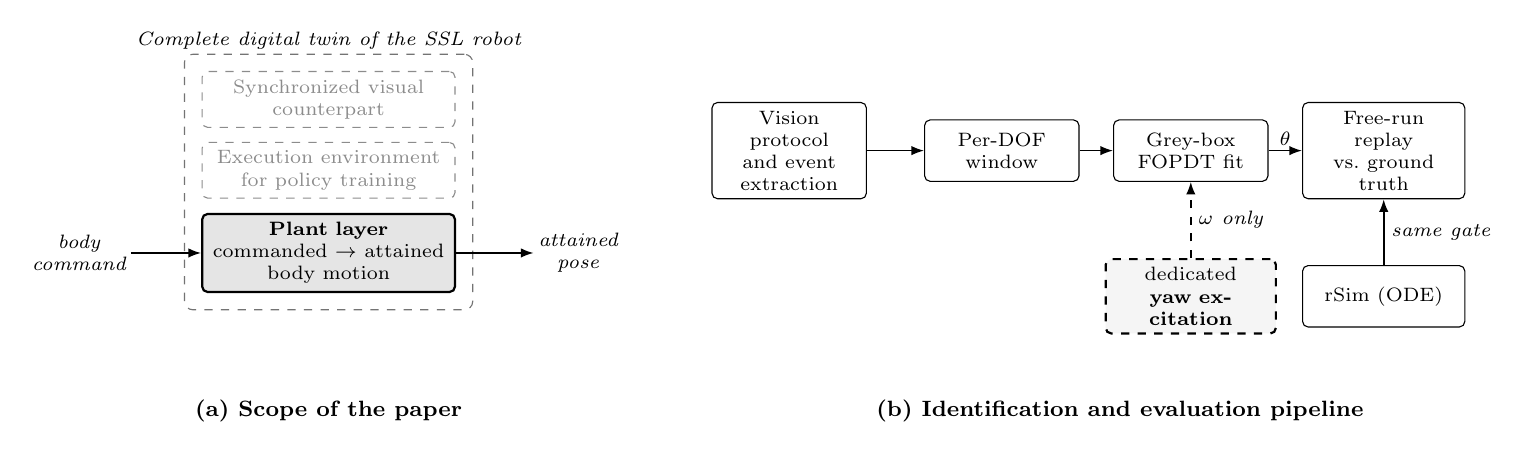
\begin{tikzpicture}[
  every node/.style={font=\scriptsize},
  blk/.style={draw, rounded corners=2pt, align=center, inner sep=3pt,
              minimum height=0.78cm},
  oos/.style={blk, dashed, draw=black!45, text=black!45, minimum height=0.62cm},
  mine/.style={blk, thick, fill=black!10, minimum height=0.86cm},
  io/.style={font=\scriptsize\itshape, align=center, inner sep=1.5pt},
  ar/.style={-{Latex[length=1.6mm]}, semithick},
  arD/.style={-{Latex[length=1.6mm]}, semithick, dashed},
  lbl/.style={font=\scriptsize\itshape, inner sep=1.5pt}
]

% ======================= PANEL (a): SCOPE ==================================
\node[oos,  text width=3.0cm] (vis)   at (2.55, 0.95)
  {Synchronized visual\\ counterpart};
\node[oos,  text width=3.0cm] (env)   at (2.55, 0.05)
  {Execution environment\\ for policy training};
\node[mine, text width=3.0cm] (plant) at (2.55,-1.00)
  {\textbf{Plant layer}\\ commanded $\rightarrow$ attained\\ body motion};

\begin{scope}[on background layer]
  \node[draw, dashed, draw=black!55, rounded corners=3pt,
        fit=(vis)(env)(plant), inner sep=6pt] (twinbox) {};
\end{scope}
\node[lbl, anchor=south] at (twinbox.north) {Complete digital twin of the SSL robot};

\node[io] (cmd) at (-0.62,-1.00) {body\\ command};
\node[io] (att) at ( 5.72,-1.00) {attained\\ pose};
\draw[ar] (cmd) -- (plant.west);
\draw[ar] (plant.east) -- (att);

% ======================= PANEL (b): PIPELINE ===============================
% Layout deliberadamente reto: uma unica linha, e os dois ramos auxiliares
% entram por BAIXO, na vertical. Nenhuma aresta cruza caixa (a versao anterior
% roteava o ramo tracejado por dentro de "Per-DOF window labeling").
\node[blk, text width=1.75cm] (p1) at ( 8.40,0.30) {Vision protocol\\ and event extraction};

%\node[blk, text width=1.75cm] (p2) at ( 9.75,0.30) {Event\\ extraction};
\node[blk, text width=1.75cm] (p3) at (11.10,0.30) {Per-DOF window};
\node[blk, text width=1.75cm] (p4) at (13.50,0.30) {Grey-box FOPDT fit};
\node[blk, text width=1.85cm] (p5) at (15.95,0.30) {Free-run replay\\ vs.\ ground truth};

\draw[ar] (p1) -- (p3);
\draw[ar] (p3) -- (p4);
\draw[ar] (p4) -- (p5) node[lbl, midway, above=0pt] {$\theta$};

% dedicated open-loop branch -- the finding, drawn as the one asymmetry
\node[blk, dashed, thick, fill=black!4, text width=1.95cm] (rot) at (13.50,-1.55)
  {dedicated \\ \textbf{yaw excitation}};
\draw[arD] (rot) -- (p4) node[lbl, midway, right=1pt] {$\omega$ only};

% baselines on the same gate
\node[blk, text width=1.85cm] (base) at (15.95,-1.55)
  {rSim (ODE)};
\draw[ar] (base) -- (p5) node[lbl, midway, right=1pt] {same gate};

% ======================= panel captions ====================================
\node[font=\footnotesize\bfseries] at ( 2.55,-3.00) {(a) Scope of the paper};
\node[font=\footnotesize\bfseries] at (12.60,-3.00) {(b) Identification and evaluation pipeline};

\end{tikzpicture}
\caption{(a) The paper delivers the plant layer of a larger digital twin: the map from commanded to attained body motion. (b) Solid path: closed-loop
competition logs. Dashed branch: the dedicated open-loop collection, which
feeds the $\omega$ channel alone. Every comparison plant is scored on the same windows, horizons and gates as the model.}
\label{fig:arch2}
\end{figure*}


This paper specifies the \emph{plant layer} of a larger digital-twin effort: a complete twin of an SSL robot also needs a synchronized visual counterpart and an execution environment in which policies can be trained, but the component that governs whether such an environment reproduces the robot's behavior at all is the map from commanded to attained body motion (Fig.~\ref{fig:arch2}a).

The pipeline runs from the league protocol stream through event extraction and per-DOF window labeling to a grey-box FOPDT fit per channel, and the resulting nine parameters drive a free-run replay scored against ground truth (Fig.~\ref{fig:arch2}b). Competition logs feed that path end to end. Every comparison plant is scored on the same windows, horizons, and statistical gates as the model.

\subsection{Per-DOF FOPDT twin}
\label{sec:method:model}
We model the robot as three decoupled single-input single-output channels, one per degree of freedom (DOF) $i\in\{v_x, v_y, \omega\}$, each a first-order-plus-dead-time (FOPDT) transfer function from commanded to attained body velocity,

\begin{equation}
  G_i(s) \;=\; \frac{K_i\, e^{-\Td{}_i s}}{\tau_i s + 1},
  \label{eq:fopdt}
\end{equation}
with per-DOF gain $K_i$, time constant $\tau_i$, and transport delay $\Td{}_i$. The inputs are the body-frame velocity commands and the outputs are the attained body velocities. The full parameter vector has fixed order $[K_{vx},\tau_{vx},\Td{}_{vx},K_{vy},\tau_{vy},\Td{}_{vy},K_{\omega},\tau_{\omega},\Td{}_{\omega}]$
(nine parameters). % source: config/ssl_robot.sldd ; config/twin_params.json ("order")
This is a \emph{behavioral} (observational) model: it targets the input-to-pose
response, not a white-box description of wheel/contact mechanics.

\subsection{Discretization and pose integration}
\label{sec:method:disc}

Identification and replay both run on a uniform grid with a step size of $\Delta t = 1/60\,\si{s}$, the nominal vision rate. Each DOF's command is delayed by a zero-order-hold (ZOH) integer shift of $m_i = \lceil \Td{}_i/\Delta t\rceil$ samples (zero before the segment start), passed through the first-order update $v_i[k] = v_i[k-1] + \alpha_i(u^{d}_i[k] - v_i[k-1])$, and scaled to the attained body velocity $\hat v_i[k] = K_i\, v_i[k]$ (instantaneous for $\tau_i \to 0$). 

\subsection{Data and pre-processing}
\label{sec:method:data}
The data are closed-loop competition logs of a single omnidirectional 4-wheeled SSL robot, decoded from the league protocol stream into per-event body-frame commands and field-frame pose at $\sim$\SI{60}{Hz}. Measured body velocity, used only for identification and for the initial condition, is obtained by smoothing the vision position with a low-order polynomial (Savitzky--Golay) filter, differentiating it by central differences, and rotating the result into the body frame. Fig.~\ref{fig:setup} shows the measurement chain: the body velocity used for identification is not read from the robot's wheel encoders but derived offline from the vision pose, both for the competition logs and for the dedicated yaw collection.\footnote{Supplementary videos (the dedicated yaw collection with the velocity extraction, and the model driven by the team's strategy): \videolink.}

%==============================================================================
% FIG. -- robot and measurement chain (camera-ready, reviewer R2: "no image of
% the robot nor of the velocity-measurement apparatus").
% Photos are optional: drop figures/robot_photo.jpg (and, if wanted,
% figures/field_photo.jpg) into the folder and they appear with the right panel
% letters; without them the figure is the measurement-chain diagram alone.
% Photo height is capped at 3 cm so that the paper stays at 6 pages (tested).
% No number here that is not in the text (60 Hz: Sec. III-C; staircase: III-D).
%==============================================================================
\IfFileExists{figures/robot_photo.jpg}{%
  \IfFileExists{figures/field_photo.jpg}{%
    \def\setupphotos{\includegraphics[width=0.47\columnwidth,height=3.0cm,keepaspectratio]{robot_photo.jpg}\hfill
      \includegraphics[width=0.47\columnwidth,height=3.0cm,keepaspectratio]{field_photo.jpg}\\[4pt]}%
    \def\setupcap{(a)~The four-wheeled omnidirectional SSL robot used in this work.
      (b)~The field and its overhead vision cameras. (c)~Measurement chain}}{%
    \def\setupphotos{\includegraphics[width=0.60\columnwidth,height=3.0cm,keepaspectratio]{robot_photo.jpg}\\[4pt]}%
    \def\setupcap{(a)~The four-wheeled omnidirectional SSL robot used in this work.
      (b)~Measurement chain}}}{%
  \def\setupphotos{}%
  \def\setupcap{Measurement chain}}
\begin{figure}[!t]
  \centering
  \setupphotos
  \resizebox{\columnwidth}{!}{%
  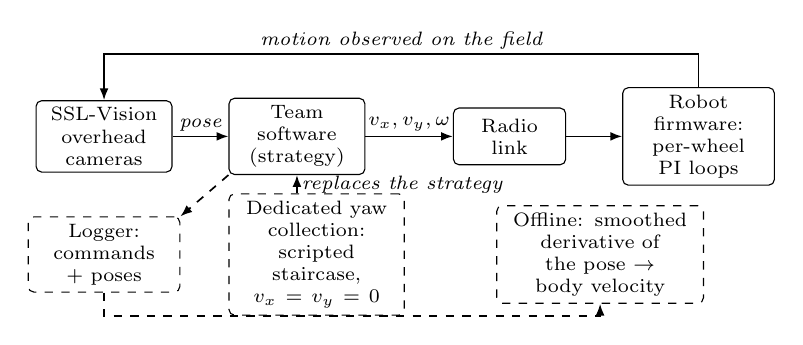
\begin{tikzpicture}[
    every node/.style={font=\scriptsize},
    blk/.style={draw, rounded corners=2pt, align=center, inner sep=2.5pt, minimum height=0.72cm},
    aux/.style={blk, dashed},
    ar/.style={-{Latex[length=1.5mm]}, semithick},
    arD/.style={-{Latex[length=1.5mm]}, semithick, dashed},
    lbl/.style={font=\scriptsize\itshape, inner sep=1.5pt}
  ]
    \node[blk, text width=1.55cm] (cam)   at (0.00,0) {SSL-Vision\\ overhead cameras};
    \node[blk, text width=1.55cm] (sw)    at (2.45,0) {Team software\\ (strategy)};
    \node[blk, text width=1.25cm] (radio) at (5.15,0) {Radio\\ link};
    \node[blk, text width=1.75cm] (robot) at (7.55,0) {Robot firmware:\\ per-wheel PI loops};
    \draw[ar] (cam) -- (sw) node[lbl, midway, above] {pose};
    \draw[ar] (sw) -- (radio) node[lbl, midway, above] {$v_x, v_y, \omega$};
    \draw[ar] (radio) -- (robot);
    \draw[ar] (robot.north) -- ++(0,0.42) -| (cam.north)
      node[lbl, pos=0.25, above] {motion observed on the field};
    \node[aux, text width=2.05cm] (stair) at (2.70,-1.50)
      {Dedicated yaw collection: scripted staircase, $v_x = v_y = 0$};
    \draw[arD] (stair.north -| sw.south) -- (sw.south) node[lbl, midway, right] {replaces the strategy};
    \node[aux, text width=1.75cm] (log) at (0.00,-1.50) {Logger:\\ commands + poses};
    \draw[arD] (sw.south west) -- (log.north east);
    \node[aux, text width=2.45cm] (off) at (6.30,-1.50)
      {Offline: smoothed derivative of the pose $\rightarrow$ body velocity};
    \draw[arD] (log.south) -- ++(0,-0.30) -| (off.south);
  \end{tikzpicture}}
  \caption[Robot and measurement chain]{\setupcap: the league vision system reports the field-frame pose at about \SI{60}{Hz}; the team software closes the loop and sends body-frame velocity commands over the radio to per-wheel loops on the robot; a logger records the commands and the poses, which is all the identification consumes. Body velocities are derived offline from the vision pose (Sec.~\ref{sec:method:data}). For the dedicated yaw collection a scripted staircase of yaw commands replaces the strategy, open loop.}
  \label{fig:setup}
\end{figure}


Logs arrive on an irregular time grid, since commands are transmitted in bursts: identification resamples every signal onto the uniform $1/60\,\si{s}$ grid, whereas the fidelity metric leaves the samples where they were recorded and defines its windows in seconds, so that no interpolation enters the reported error.
The dataset comprises $46$ events across four motion labels (\texttt{front\_to\_back}, \texttt{side\_to\_side}, \texttt{shoot\_to\_goal}, \texttt{square}); a frozen list of $10$ events is held out and was not used for fitting.

Throughout, \emph{fit} measures how much of the variation in the measured signal the model reproduces, on events the fit never saw:
\begin{equation}
  \mathrm{fit} = 100\left(1 -
  \frac{\lVert y - \hat{y}\rVert_2}{\lVert y - \bar{y}\rVert_2}\right)\ [\%],
  \label{eq:fit}
\end{equation}
where $y$ is the measured body velocity of the degree of freedom being identified, $\hat{y}$ is the model's output when driven by the commands alone, and $\bar{y}$ is the mean of $y$.

\subsection{Identification}
\label{sec:method:id}
Each translational DOF is identified independently as a P1D (FOPDT) model by prediction-error minimization, with an event-level hold-out. The excitation diagnostic selects the cleanest source label per DOF: $v_x$ from \texttt{front\_to\_back} and $v_y$ from \texttt{side\_to\_side} (command-to-velocity cross-correlation $\approx 0.99$).
Yaw is instead identified from a dedicated open-loop collection, with the same model structure and the same estimator, because the competition logs carry too little yaw excitation to support the fit. The dedicated dataset is single-session and single-robot with $v_x=v_y=0$: an alternating-sign staircase of commanded yaw rates $\{0.25,0.5,1,2.5,5\}\,\si{rad/s}$, $\sim\SI{10}{s}$ per step.

\subsection{Frames, constants and replication}
\label{sec:method:geometry}
Commands and attained velocities live in the \emph{body} frame: $v_x$ longitudinal, $v_y$ lateral, $\omega$ yaw rate about the upward $z$ axis, counter-clockwise positive. Pose is integrated in the \emph{field} frame as $\dot{X} = v_x\cos\theta - v_y\sin\theta$, $\dot{Y} = v_x\sin\theta + v_y\cos\theta$, with $\theta$ unwrapped.
Per-wheel geometry converts the firmware's per-wheel motor threshold ($\SI{1.567}{rad/s}$) into a body yaw rate for Sec.~\ref{sec:results:omega}, through the ratio of the center-to-wheel-contact radius $R=\SI{0.0796}{m}$ to the wheel radius $r=\SI{0.0295}{m}$.

\subsection{Free-run replay and multi-horizon metric}
\label{sec:method:metric}
Fidelity is measured in \emph{free-run}: segments are cut into overlapping windows at a fixed stride, each re-anchored to the true $\SEtwo$ pose at its anchor $t_0$ and rolled out to $H_{\max}=90$ samples ($\SI{1.5}{s}$) driven only by the command stream. The Euclidean position error $\epos(w,h)$ and the wrapped absolute heading error $\eang(w,h)$ at $h\in\{6,12,24,42,60,90\}$ samples ($\{0.1,0.2,0.4,0.7,1.0,1.5\}\,\si{s}$), with reference horizon $h_{\mathrm{ref}}=24$ ($\SI{0.4}{s}$) are reported separately. $\epos$ is the claim of this paper; $\eang$ is reported but bounded by the population of rotation-rich windows available (Sec.~\ref{sec:results:bins}).
% source: config/metrics.json (horizons, h_ref)

\subsection{Baselines}
\label{sec:method:baselines}
We compare the twin against two baselines under the \emph{same} windows, horizons, and gate. The first is an \emph{ideal-kinematics} plant in which the attained body velocity equals the command instantaneously (no gain, lag, or delay), integrated by the same trapezoidal scheme. The second is \textbf{rSim}, the ODE-based physics engine of the rSoccer environment, run with its stock robot parameters and no fitting to these logs, so the comparison is between a plant fitted to this robot and an untuned engine; it is reported as context, not as the primary comparison. The recorded body-frame commands enter it directly as body-velocity setpoints, with no motion controller in between, and it is stepped in \SI{1}{ms} substeps interpolated back onto the $1/60\,\si{s}$ grid. rSim has no velocity setter at reset, so each window warms it up over the $15$ real pre-anchor commands before a rigid $\SEtwo$ re-anchor at $t_0$; the dead-time term of the model has no counterpart in it.
% source: src/dtssl/models/rsim.py (robosim.SSL with stock parameters; wheel_speed=False, body-velocity action;
%   sub_ms=1 with linear interpolation onto the 1/60 s grid; warm-up over LW=15 pre-anchor commands, rigid SE(2) re-anchor)




\section{Results}
\label{sec:results}

\subsection{Identified model}
\label{sec:results:id}

Table~\ref{tab:sysid} reports the per-DOF parameters. Both translational
channels identify as fast FOPDT models, with hold-out fit $86.7\%$ ($v_x$) and $87.1\%$ ($v_y$); against the previous, slower parameters, they improve every event-by-horizon cell of the $\SEtwo$ gate. Yaw is identified from a separate open-loop dataset at $71.1\%$.

%==============================================================================
% TABLE: identified per-DOF FOPDT parameters + hold-out fit.
% Source: config/twin_params.json ; models/sysid_vxvy_v2.mat ;
%         models/sysid_omega_rotate_v1.mat ; results/identificacao_omega_20260724.md ;
%         docs/RELATORIO_TECNICO_DESENVOLVIMENTO.md sec.5 ; CHANGELOG 2026-06-14 / 2026-07-24.
%==============================================================================
\begin{table}[t]
  \caption{Identified per-DOF FOPDT parameters and hold-out fit. All three
  channels are identified (no placeholder); $\omega$ uses a dedicated
  open-loop rotation-only collection (see Sec.~\ref{sec:results:omega}), not
  the closed-loop competition logs used for $v_x,v_y$.}
  \label{tab:sysid}
  \centering
  \begin{tabular}{lcccc}
    \toprule
    DOF & $K$ & $\tau$ (s) & $\Td$ (s) & hold-out fit \\
    \midrule
    $v_x$     & 1.119 & 0.072 & 0.069 & 86.7\,\% \\
    $v_y$     & 1.052 & 0.127 & 0.056 & 87.1\,\% \\
    $\omega$  & 1.002 & 0.083 & 0.089 & 71.1\,\% \\
    \bottomrule
  \end{tabular}
  \\[2pt]
  \raggedright\footnotesize Fit is Eq.~\ref{eq:fit}, averaged over hold-out
  events. Because $v_x$ has a single hold-out event, we also ran
  leave-one-event-out over all events of each translational label: $v_x$ gives
  $84.3\pm2.0$~p.p.\ over 4 folds and $v_y$ $82.8\pm2.7$~p.p.\ over 13, with the
  refitted gain within $0.015$ of the promoted value in both cases. No parameter
  intervals are reported: see Sec.~\ref{sec:results:omega}.
  % source: results/loo_translational_20260810_1743.md — refit completo por
  %   dobra, sem alterar o modelo promovido. ATENCAO: o artefato _1742 e a
  %   execucao QUEBRADA (posicao em mm tratada como m, K~1073, tau negativo);
  %   foi descartado. Citar sempre _1743.
\end{table}


\begin{figure}[!t]
  \centerline{\includegraphics[width=0.70\columnwidth]{omega_stepresponse_en.png}}
  \caption{Measured vs.\ simulated yaw rate on the dedicated open-loop
  staircase (one training, two hold-out steps). Same model structure and
  identification tooling as on the competition logs; only the excitation regime
  differs.}
  \label{fig:fits}
\end{figure}

\subsection{Motion distribution of the hold-out}
\label{sec:results:bins}
The hold-out windows are overwhelmingly translation-dominated: of $265$ dense windows ($49$ non-overlapping), $264$ fall in the translation bin ($99.6\%$), one is rotation-dominated, and none are mixed. Re-classifying after $\omega$ was identified reproduces the same $264/1/0$ split and leaves both other bins with $N_{\mathrm{indep}}=0$, now for lack of rotation-rich competition windows rather than for lack of a yaw model.

\begin{figure*}[!t]
  \centerline{\includegraphics[width=0.86\textwidth]{main_result_en.png}}
  \caption{(a) Median free-run position error against horizon on
  translation-dominated hold-out windows, for the FOPDT model, ideal kinematics, and an untuned rSim. The two baselines cross near $\SI{1}{s}$. (b) The same comparison resolved by event at $h_{\mathrm{ref}}$: each line is one of the ten hold-out events, and the model is lower in all ten.
  }
  \label{fig:main}
\end{figure*}

\subsection{Translational fidelity}
\label{sec:results:rsim}

Ideal kinematics is the primary comparator: both plants run in the same
harness, start from the same measured body velocity and are scored on the same
windows, so the model is the only difference. Its median position error is
lower at every horizon (Fig.~\ref{fig:main}, Table~\ref{tab:three}):
$\SI{0.039}{m}$ against $\SI{0.101}{m}$ at $h_{\mathrm{ref}}$, and
$\SI{0.119}{m}$ against $\SI{0.291}{m}$ at $\SI{1.5}{s}$. For scale, the robot
covers about $\SI{0.4}{m}$ within $h_{\mathrm{ref}}$ and its contact diameter is
$\SI{0.16}{m}$: the baseline misses by two thirds of a robot, the model by a
quarter.

The hold-out is ten events, $\SI{73.5}{s}$ of scored motion. Windows from one
event share robot, surface, session and controller, so we take the \emph{event}
as the unit of analysis. The model wins all ten, by a median of
$+\SI{0.069}{m}$ (one-sided Wilcoxon $p = 9.8\times10^{-4}$, the smallest value
attainable at $n = 10$); the pre-registered window-level test over the $49$ non-overlapping windows
agrees and is the less conservative of the two.\ifkeeptrajfig{} Fig.~\ref{fig:trajlabels} shows the same comparison in the trajectory domain, one panel per motion label.\fi
% source: results/gate_window_vs_event_20260810_1743.md (window n = 49, event n = 10)

%==============================================================================
% TABELA: e_pos e e_ang das TRES plantas por horizonte (bin translacional).
% Criada 2026-08-10 em resposta a B3 da revisao V2 ("o resultado principal do
% artigo nao tem figura nem tabela") e a C6 (o artigo afirmava que o e_ang do
% twin excede o do rSim em horizontes longos sem nunca dar o numero do rSim).
% Fonte: results/epos_eang_three_models_20260810_1022.md, gerada por
% scripts/epos_eang_three_models.py sobre as mesmas janelas do gate.
% NOTA: os numeros de e_ang REFUTAM a afirmacao anterior do artigo -- o modelo
% tem heading MENOR que o rSim em TODOS os horizontes. Texto corrigido.
%==============================================================================
\begin{table}[t]
  \caption{Median free-run error on translation-dominated hold-out windows.
  Position error in meters, heading error in radians. The model is lowest in
  both quantities at every horizon; the two baselines cross in position near
  $\SI{1}{s}$.}
  \label{tab:three}
  \centering
  \setlength{\tabcolsep}{4pt}
  \begin{tabular}{ccccccc}
    \toprule
    & \multicolumn{3}{c}{$\epos$ (m)} & \multicolumn{3}{c}{$\eang$ (rad)} \\
    \cmidrule(lr){2-4}\cmidrule(lr){5-7}
    $h$ (s) & model & ideal & rSim & model & ideal & rSim \\
    \midrule
    0.10 & \textbf{0.008} & 0.026 & 0.057 & \textbf{0.013} & 0.023 & 0.026 \\
    0.20 & \textbf{0.018} & 0.050 & 0.092 & \textbf{0.031} & 0.044 & 0.046 \\
    0.40 & \textbf{0.039} & 0.101 & 0.129 & \textbf{0.044} & 0.067 & 0.064 \\
    0.70 & \textbf{0.062} & 0.152 & 0.174 & \textbf{0.063} & 0.076 & 0.079 \\
    1.00 & \textbf{0.092} & 0.217 & 0.213 & \textbf{0.073} & 0.092 & 0.086 \\
    1.50 & \textbf{0.119} & 0.291 & 0.289 & \textbf{0.090} & 0.095 & 0.094 \\
    \bottomrule
  \end{tabular}
\end{table}


\subsubsection{What produces the improvement}
We switch each of $\{K,\tau,\Td\}$ off in every combination and average over all
orderings, so no term is credited merely for being enabled first. Of the
$\SI{0.062}{m}$ separating the two plants at $h_{\mathrm{ref}}$, the time
constant accounts for $55\%$, the dead time for $43\%$ and the gain for $2\%$.
Lag and delay are comparable contributors; the gain is irrelevant.

\subsubsection{The role of the measured initial velocity}
Both plants are seeded with the measured body velocity, but only the dynamic one
can carry it forward, and neither ingredient works alone. Extrapolating that
velocity at constant speed, ignoring the commands, gives $\SI{0.160}{m}$;
running the model from rest gives $\SI{0.114}{m}$. Both are worse than ideal
kinematics, and only the combination reaches $\SI{0.039}{m}$. We treat the
measured velocity as part of the model interface rather than privileged
information, since a twin running alongside the robot has that estimate;
re-deriving it with a strictly causal difference raises both errors but
\emph{widens} the gap, so the verdict does not rest on it.

\subsubsection{The untuned ODE simulator}
rSim reaches $\SI{0.129}{m}$ at $h_{\mathrm{ref}}$, so even the zero-parameter baseline outperforms it. Giving it the model's dead time widens rather than closes the gap.

\subsubsection{Heading error}
The rotation and mixed bins lack a scorable population
(Sec.~\ref{sec:results:bins}), so heading carries no verdict. Descriptively
(Table~\ref{tab:three}), the model's median $\eang$ is the lowest of the three
plants at every horizon, but the margin shrinks from roughly half the
baselines' at $\SI{0.1}{s}$ to within $\SI{0.005}{rad}$ of both by
$\SI{1.5}{s}$. The position advantage does not transfer to heading in the same
proportion, which is consistent with yaw being the channel the competition logs
cannot constrain.

\subsection{Yaw identifiability is a function of excitation regime}
\label{sec:results:omega}

\ifkeeptrajfig
\begin{figure*}[!t]
  \centerline{\includegraphics[width=0.98\textwidth]{trajectory_by_label_en.png}}
  \caption{Free-run trajectory overlays, one per motion label, over a
  $\SI{1.5}{s}$ window re-anchored at the black dot. For each label we show the
  window with the largest margin of the model over the better of the two
  comparison plants, so these are per-label best cases rather than typical
  windows; the median-window overlay and the full distributions are in
  Fig.~\ref{fig:main} and Table~\ref{tab:three}. Panel titles give the
  end-of-window position error of each plant.}
  \label{fig:trajlabels}
\end{figure*}
\fi

The problem is visible in the logs before any model is fitted. Regressing the
measured body velocity on the command, aligned by its dead time, the command
explains $96\%$ of the variance for $v_x$ and $94\%$ for $v_y$, but only $56\%$
for $\omega$: nearly half the rotation the cameras see in play is not
attributable to the yaw command.

Fitting the same structure to the highest-rotation competition events gives
$K_\omega = 1.378$ and a hold-out fit of $44.8\%$, below the pre-registered
$60\%$ gate. Using it also \emph{worsens} free-run position, because a gain
above unity amplifies accumulated heading drift, so it is not promoted.

\subsubsection{Why the logs cannot constrain yaw}
The firmware clamps each \emph{wheel} setpoint below $\SI{1.567}{rad/s}$, after
the command kinematics. Converted to body yaw rate that threshold sits at
$0.58$--$0.60\,\si{rad/s}$, and $94.3\%$ of commanded yaw samples in the logs
fall below it. The statistic is easy to misread: it does not mean yaw is
switched off. In play the wheels are already turning because of translation, so
among those samples the median per-wheel translational setpoint is $15\times$
the clamp and only $2.2\%$ are fully clamped. The yaw command is not suppressed
but \emph{diluted}, contributing a median of $1.0\%$ of what each wheel is asked
to do. What the actuators receive in competition is $99\%$ translation.

\subsubsection{The same structure on dedicated data}
A short dedicated open-loop collection removes the dilution: with
$v_x = v_y = 0$ the yaw command becomes the sole actuation. Identified with the
\emph{same} structure and tooling (Fig.~\ref{fig:fits}), it gives
$K_\omega = 1.002$, $\tau_\omega = \SI{0.083}{s}$, $\Td{}_\omega = \SI{0.089}{s}$
and a hold-out fit of $71.1\%$, above the gate. Scored against the same fixed
placeholder yaw channel ($K=1$, $\tau=\SI{0.1}{s}$, $\Td=0$) on the same competition population, the closed-loop estimate is
worse at every horizon and the open-loop one better, so the verdict inverts
under identical tooling.
% Limitations are a subsection of the Discussion (05); 06_limitations.tex is not built.
%==============================================================================
% DISCUSSION + LIMITATIONS — FUNDIDAS numa seção só (2026-08-10, pedido do
% autor; corte 9->6 páginas). A Seção VI separada foi eliminada e o arquivo
% 06_limitations.tex saiu do build.
% GUARDRAIL: nenhuma limitação foi REMOVIDA. Todas as sete continuam
% enunciadas, agora em um parágrafo denso: amostra pequena / sessão e robô
% únicos / contraste não single-factor / estimadores closed-loop não tentados /
% Ljung-Box / constantes cinemáticas / rSim não sintonizado + baseline ideal +
% mismatch de velocidade inicial / escopo de um único dataset e grade irregular.
% O detalhamento longo permanece em docs/BACKLOG_EXTENSAO_JINT.md item A.
%==============================================================================
\section{Discussion}
\label{sec:discussion}

\subsection{Identifiability is a property of the data, not the DOF}
\label{sec:discussion:inversion}
The central finding is not that yaw is harder to model than translation, but
that the \emph{same} structure and tooling give opposite verdicts depending on
the excitation regime: on closed-loop logs the yaw P1D meets none of the
acceptance criteria, while on a small dedicated collection it passes every
pre-registered gate with near-unity gain. Nothing in the pipeline distinguishes
the DOFs; only the data does, since those logs excite $v_x,v_y$ persistently
while the yaw command is a median $1\%$ of the per-wheel actuation.

The closed-loop gain estimate is not merely imprecise; it is wrong in the same
direction across two independent attempts, a direct high-rotation fit and a
regime-restricted linear fit. The dilution result of
Sec.~\ref{sec:results:omega} says what that estimator is actually fitting:
with the yaw command at about $1\%$ of the per-wheel setpoint, it explains only
$56\%$ of the variance of the measured rotation, the remainder plausibly coming
from slip, contact and traction asymmetry generated by the translational motion. Regressing
measured yaw on commanded yaw is then dominated by whatever correlates with the
command, and under feedback the controller issues yaw precisely in response to
those disturbances, which is the textbook closed-loop identification
hazard~\cite{gustavsson1977identification,vandenhof1998closedloop,forssell1999closedloop}.
This removes the reading that the actuation threshold simply switches yaw off,
since it engages in only ${\sim}2\%$ of samples, and replaces it with something
measurable. It does not isolate feedback from dilution, because the dedicated
collection removes both at once.

\subsection{Limitations}
\label{sec:limitations}
% CORTE 2026-08-10 (9->6 pag.): parágrafo enxugado ~40%. GUARDRAIL mantido --
% todas as sete limitações continuam enunciadas, apenas sem detalhamento.
The yaw fit rests on six events from a single session, with no fine amplitude
sweep, so its threshold is an interval; all data come from one robot, one
surface and one hold-out split, and pre-registration and deterministic
re-execution mitigate but do not replace replication. The two yaw campaigns
differ in loop topology, yaw-to-translation ratio and session at once, so
separating the last two would need an open-loop arm with translation
superimposed, which we did not collect; nor did we attempt the closed-loop-aware
estimators (instrumental-variable, two-stage, joint input--output) the cited
literature proposes. Ljung--Box rejects residual whiteness for both yaw fits,
which the smoothing differentiator explains and which is why no parameter
intervals are reported. The firmware and CAD radius ratios still differ by
${\sim}3.3\%$. On evaluation, $99.6\%$ of hold-out windows are
translation-dominated, so rotational fidelity is not validated; the heading
advantage all but vanishes by $\SI{1.5}{s}$ (Table~\ref{tab:three}), so the
position claim does not transfer to heading in the same proportion; and the
rSim comparison remains fitted-versus-untuned and confounded by
% FIX 2026-08-10 (revisao V3, objecao 3a): esta frase ainda dizia que o e_ang do
% modelo EXCEDE o do rSim, contradizendo a Tabela III e o texto de IV-C, ja
% corrigidos quando o e_ang do rSim foi finalmente medido.
initial state, which the matched-delay ablation narrows but does not remove.
The model is also deliberately simple, and three simplifications bound where it
applies. The channels are decoupled: no term maps a translational command into
yaw or a yaw command into translation, although part of the $44\%$ of the
measured rotation that the yaw command leaves unexplained in play is plausibly
translation-induced yaw (slip, contact and traction asymmetry), which is exactly
what a coupled model would have to capture; a coupled (MIMO) identification on
the same data is the natural next step and is not attempted here. The plant is
linear, with no saturation, acceleration limit or dead zone: it is fitted and
scored inside the envelope of the logs, where the commanded speed exceeds
$\SI{2.9}{m/s}$ in only $0.01\%$ of the competition samples and the dedicated
yaw steps peak at about a quarter of the per-wheel PWM limit, so its validity
in aggressive or mixed-motion regimes is unverified. Slip enters only through
the identified gains and lags, never as a state.
% source: results/excitation_per_dof_20260810_1022.md (w: R^2 = 0.557);
%   results/closed_loop_stats_20260907_2137.md (competition pool, 46 events, 22812 samples at 60 Hz:
%   |v| > 2.9 m/s in 0.01 %, max |v| 2.91 m/s); results/qc_rotate_20260724_125828.md sec. 6
%   (max |PWM| 20.38 at +-5 rad/s vs the firmware limit +-80, 25 %); config/robot_limits.json
%   ("the published behavioral plant has NO saturation/acceleration limit"; deadzone off by default).
% source: results/identificacao_omega_20260724.md Etapa 4 ; qc_rotate_20260724_125828.md ;
%   config/robot_geometry.json ; docs/PREREGISTRO_OMEGA_20260724.md ;
%   results/window_errors_eang_summary_20260731_023856.md ;
%   results/eval_twin_vs_rsim_mode{A,B}_20260617_*.md


%==============================================================================
% CONCLUSION — resumida 2026-08-10 (pedido do autor, corte 9->6 páginas).
% De ~3 blocos para 2 parágrafos curtos. Availability preservada (fecha C10);
% Future work reduzido a uma frase por direção.
%==============================================================================
\section{Conclusion and Future Work}
\label{sec:conclusion}

This paper presented a per-DOF FOPDT model of an omnidirectional SSL robot, identified mostly from closed-loop competition logs, which attains validated translational fidelity: over $\SI{73.5}{s}$ of scored hold-out motion it lowers the median position error of a baseline in all ten hold-out events, halving it at the reference horizon, with the improvement attributable in comparable parts to the time constant and the dead time, and only in combination with the measured initial velocity.
Yaw needed a short dedicated open-loop campaign, after characterizing why the logs cannot support it: during play the yaw command carries a median $1\%$ of the per-wheel actuation and explains only $56\%$ of the variance of the measured rotation. Code, configurations, and both datasets are released at
\repolink, with instructions to reproduce every number above. Future work embeds this plant in a full digital twin inside a robot-learning environment such as Isaac Sim or MuJoCo \cite{machado2025planning}, and adds a rotation-rich validation distribution, an open-loop arm with translation superimposed, and cross-robot replication.



\section*{Acknowledgment}
REPLACE-ME: funding agencies and grant numbers; the Rob\^{o}CIn team; who ran the
dedicated yaw collection and who produced the CAD model.

\bibliographystyle{IEEEtran}
\bibliography{refs/references}

\end{document}
